\documentclass[12pt,a4paper,bibliography=totocnumbered,listof=totocnumbered]{scrartcl}
\usepackage[ngerman]{babel}
\usepackage[utf8]{inputenc}
\usepackage{amsmath}
\usepackage{amsfonts}
\usepackage{amssymb}
\usepackage{csquotes}
\usepackage{graphicx}
\usepackage{fancyhdr}
\usepackage{float}
\usepackage{tabularx}
\usepackage{geometry}
\usepackage{setspace}
\usepackage[right]{eurosym}
\usepackage[printonlyused]{acronym}
%\usepackage{subfig}
\usepackage{floatflt}
\usepackage[usenames,dvipsnames]{color}
\usepackage{colortbl}
\usepackage{paralist}
\usepackage{array}
\usepackage{subcaption}
\usepackage{wrapfig}
\usepackage{titlesec}
\usepackage{parskip}
\usepackage[right]{eurosym}
\usepackage{picins}
\usepackage[subfigure,titles]{tocloft}
\usepackage[pdfpagelabels=true]{hyperref}
\usepackage[export]{adjustbox}

\usepackage{listings}
\lstset{basicstyle=\footnotesize, captionpos=b, breaklines=true, showstringspaces=false, tabsize=2, frame=lines, numbers=left, numberstyle=\tiny, xleftmargin=2em, framexleftmargin=2em}
\makeatletter
\def\l@lstlisting#1#2{\@dottedtocline{1}{0em}{1em}{\hspace{1,5em} Lst. #1}{#2}}
\makeatother

\geometry{a4paper, top=27mm, left=30mm, right=20mm, bottom=35mm, headsep=10mm, footskip=12mm}

\hypersetup{unicode=false, pdftoolbar=true, pdfmenubar=true, pdffitwindow=false, pdfstartview={FitH},
	pdftitle={Learning Diary},
	pdfauthor={Christian Neubauer },
	pdfsubject={Independent Coursework},
	pdfcreator={\LaTeX\ with package \flqq hyperref\frqq},
	pdfproducer={pdfTeX \the\pdftexversion.\pdftexrevision},
	pdfkeywords={Abschlussarbeit},
	pdfnewwindow=true,
	colorlinks=true,linkcolor=black,citecolor=black,filecolor=magenta,urlcolor=black}
\pdfinfo{/CreationDate (D:20110620133321)}

\begin{document}

\titlespacing{\section}{0pt}{12pt plus 4pt minus 2pt}{-6pt plus 2pt minus 2pt}

% Kopf- und Fusszeile
\renewcommand{\sectionmark}[1]{\markright{#1}}
\renewcommand{\leftmark}{\rightmark}
\pagestyle{fancy}
\lhead{}
\chead{}
\rhead{\thesection\space\contentsname}
\lfoot{Independent Coursework}
\cfoot{}
\rfoot{\ \linebreak Seite \thepage}
\renewcommand{\headrulewidth}{0.4pt}
\renewcommand{\footrulewidth}{0.4pt}

% Vorspann
\renewcommand{\thesection}{\Roman{section}}
\renewcommand{\theHsection}{\Roman{section}}
\pagenumbering{Roman}

% ----------------------------------------------------------------------------------------------------------
% Titelseite
% ----------------------------------------------------------------------------------------------------------
\thispagestyle{empty}
\begin{center}
	
\includegraphics[scale=1]{Bilder/HTW_Logo_rgb.png}\\
	\vspace*{2cm}
	\Large
	\textbf{Fachbereich 4}\\
	\textbf{Informatik, Kommunikation und Wirtschaft}\\
	\vspace*{2cm}
	\Huge
	\textbf{Independent Coursework I}\\
	\vspace*{0.5cm}
	\large
	\vspace*{1cm}
	\textbf{Umsetzung einer iOS Applikation basierend auf dem Masterprojekt Neeedo.com mit Swift }\\
	\vspace*{2cm}
	
	\vfill
	\normalsize
	\newcolumntype{x}[1]{>{\raggedleft\arraybackslash\hspace{0pt}}p{#1}}
	\begin{tabular}{x{6cm}p{7.5cm}}
		\rule{0mm}{5ex}\textbf{Autor:} & Christian Neubauer\newline Matr.Nr. 547617 \\ 
		\rule{0mm}{5ex}\textbf{Prüfer:} & Prof. Dr. Jung \\ 
		\rule{0mm}{5ex}\textbf{Abgabedatum:} & 24.03.2016 \\ 
	\end{tabular} 
\end{center}
\pagebreak

% ----------------------------------------------------------------------------------------------------------
% Verzeichnisse
% ----------------------------------------------------------------------------------------------------------
% TODO Typ vor Nummer
\renewcommand{\cfttabpresnum}{Tab. }
\renewcommand{\cftfigpresnum}{Abb. }
\settowidth{\cfttabnumwidth}{Abb. 10\quad}
\settowidth{\cftfignumwidth}{Abb. 10\quad}

\titlespacing{\section}{0pt}{12pt plus 4pt minus 2pt}{2pt plus 2pt minus 2pt}
\singlespacing
\rhead{INHALTSVERZEICHNIS}
\renewcommand{\contentsname}{II Inhaltsverzeichnis}
\phantomsection
\addcontentsline{toc}{section}{\texorpdfstring{II \hspace{0.35em}Inhaltsverzeichnis}{Inhaltsverzeichnis}}
\addtocounter{section}{1}
\tableofcontents
\pagebreak
\rhead{VERZEICHNISSE}
\listoffigures
\pagebreak
%\listoftables
%\pagebreak
%\renewcommand{\lstlistlistingname}{Listing-Verzeichnis}
%{\labelsep2cm\lstlistoflistings}
\pagebreak
% ----------------------------------------------------------------------------------------------------------
% Abkürzungen
% ----------------------------------------------------------------------------------------------------------
\section{Abkürzungsverzeichnis}
\begin{acronym}[OSGi] % längste Abkürzung steht in eckigen Klammern
	\setlength{\itemsep}{-\parsep} % geringerer Zeilenabstand
	\acro{MOOC}{Massive Open Online Course}
	\acro{IC}{Independent Coursework}
	\acro{RWD}{Responsive Web Design}
	\acro{CPL}{Characters per line}
\end{acronym}
\newpage

% ----------------------------------------------------------------------------------------------------------
% Inhalt
% ----------------------------------------------------------------------------------------------------------
% Abstände Überschrift
\titlespacing{\section}{0pt}{12pt plus 4pt minus 2pt}{-6pt plus 2pt minus 2pt}
\titlespacing{\subsection}{0pt}{12pt plus 4pt minus 2pt}{-6pt plus 2pt minus 2pt}
\titlespacing{\subsubsection}{0pt}{12pt plus 4pt minus 2pt}{-6pt plus 2pt minus 2pt}

% Kopfzeile
\renewcommand{\sectionmark}[1]{\markright{#1}}
\renewcommand{\subsectionmark}[1]{}
\renewcommand{\subsubsectionmark}[1]{}
\lhead{Kapitel \thesection}
\rhead{\rightmark}

\onehalfspacing
\renewcommand{\thesection}{\arabic{section}}
\renewcommand{\theHsection}{\arabic{section}}
\setcounter{section}{0}
\pagenumbering{arabic}
\setcounter{page}{1}


% ----------------------------------------------------------------------------------------------------------
% Einleitung
% ----------------------------------------------------------------------------------------------------------
\section{Einleitung}
\subsection{Ausgangslage}

Im Wintersemester 2014/15 und Sommersemester '15 entstand in Zusammenarbeit mit der Firma Commercetools das Masterprojekt \enquote{neeedo.com}. 
Die Idee dieses Projektes wurde als next-generation e-Commerce tituliert und sollte, alternative Ideen und moderne Technologien in das e-Commerce Umfeld bringen. 

\subsubsection{Die Firma Commercetools}  

Die Firma Commercetools entwickelt und vertreibt die e-Commerce-Plattform "Sphere.io", heute "commerceTools platform". Dies ist eine Commerce-as-a-Service Platform, die es dem Anwender erlaubt auf einfache Weise einen (Online-) Shop zu erstellen und zu verwalten. F"ur diese Plattform steht ebenfalls eine Entwickler-API zur Verf"ugung, auf der dieses Projekt aufbaut.

\subsubsection{Das Ergebnis}

Das Ergebnis des Projektes \enquote{neeedo.com} war eine Verkaufsplattform, in der die Idee der Suche/Biete Karten, bekannt vom klassischen \enquote{Schwarzen Brett}, aufgegriffen und in einem modernen Gewand pr"asentiert wird. 
Es wurden dabei neue Ans"atze f"ur das Suchen und Anbieten von Produkten umgesetzt. Ein intelligentes Matching-System hilft den Nutzern dabei das zu finden was sie suchen.

Umgesetzt wurde das Projekt mithilfe einer selbst entwickelten Scala/Play-API, die die Verbindung zum Commercetools-Service herstellt, der die Datenhaltung und weitere interne Funktionen bereitstellt. 
In dieser API finden zudem alle Operationen zum Suchen und Erstellen von Artikeln statt, sowie das Matching und andere Funktionen. 
Welche Funktionen von der API genau erf"ullt werden wird in der Umsetzung ersichtlich.

Auf dieser API aufbauend wurden eine WebApplikation und eine native Android Applikation umgesetzt, die als Schnittstelle zum Benutzer dienen. 

\subsection{Idee}

W"ahrend des Projekts stand immer wieder die Entwicklung einer zus"atzlichen iOS Applikation im Raum. 
Diese wurde aber schlussendlich nicht umgesetzt.

Dies soll nun im Rahmen dieses \enquote{Independent Courseworks} nachgeholt werden. 

Da, wie die Analyse dieser zeigen wird, markante Schw"achen in der Usability der Android Applikation existieren, soll ein Schwerpunkt dieser Arbeit sein diese zu verbessern bzw. ein neues Konzept zu entwickeln. Dies ist auch notwendig, da die aktuellen iOS-Ger"ate abweichende Verhalten im Vergleich zu Android Ger"aten aufweisen.

% ----------------------------------------------------------------------------------------------------------
% Usability
% ----------------------------------------------------------------------------------------------------------
\section{Usability Analyse}

Da dieses Projekt auf Grundlage der Ergebnisse aus dem Projekt neeed.com entsteht, soll zuerst der IST-Stand analysiert werden.

Zuerst soll eine Betrachtung der bestehende  Android - Applikation  Aufschluss dar"uber geben was Positiv ist und wo Verbesserungen an der Usability angebracht sind. 

\subsection{IST - Stand}

Bisher besteht das Projekt neeedo.com aus einer Android Applikation, einer WebApp und der verbindenden AP.  
Die Android Applikation ist von Verhalten und Optik her, an die Webapplikation angelehnt, und um Elemente anderer bekannter mobiler Applikationen erweitert um die geplanten Funktionen umzusetzen. 

Anhand verschiedener Screenshots soll im folgenden dargestellt werden was positiv/ negativ ist  und welche L"osungen als Verbesserungen umgesetzt werden k"onnten. 

\subsubsection{Login}
\begin{figure}[H]
 
\begin{subfigure}{0.5\textwidth}
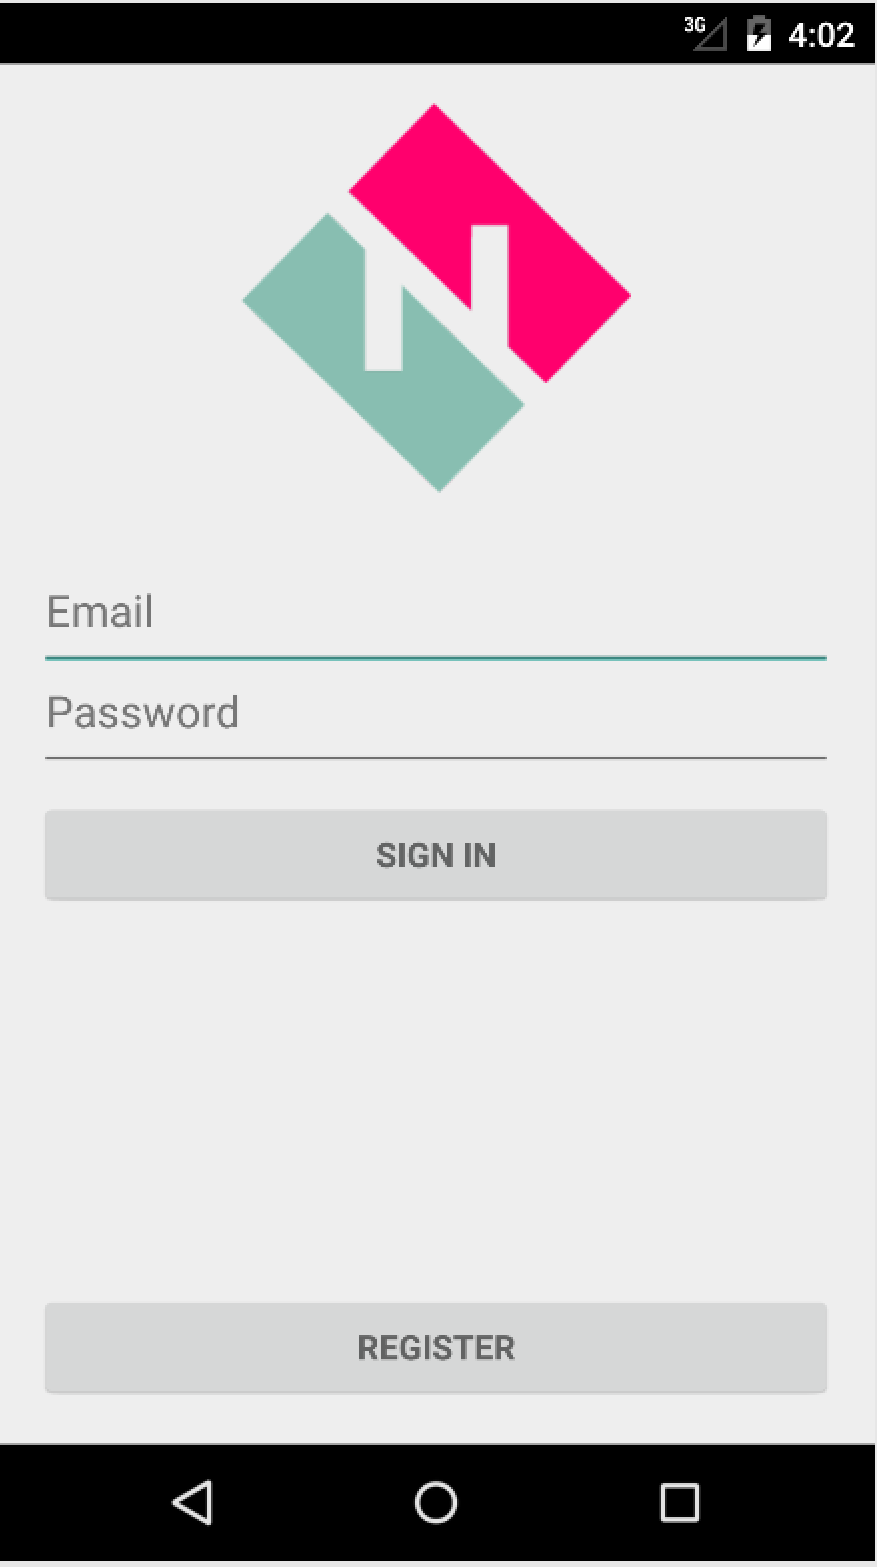
\includegraphics[width=0.9\linewidth]{./Bilder/logIn.png} 
\caption{LogIn Screen}
\label{fig:login}
\end{subfigure}
\begin{subfigure}{0.5\textwidth}
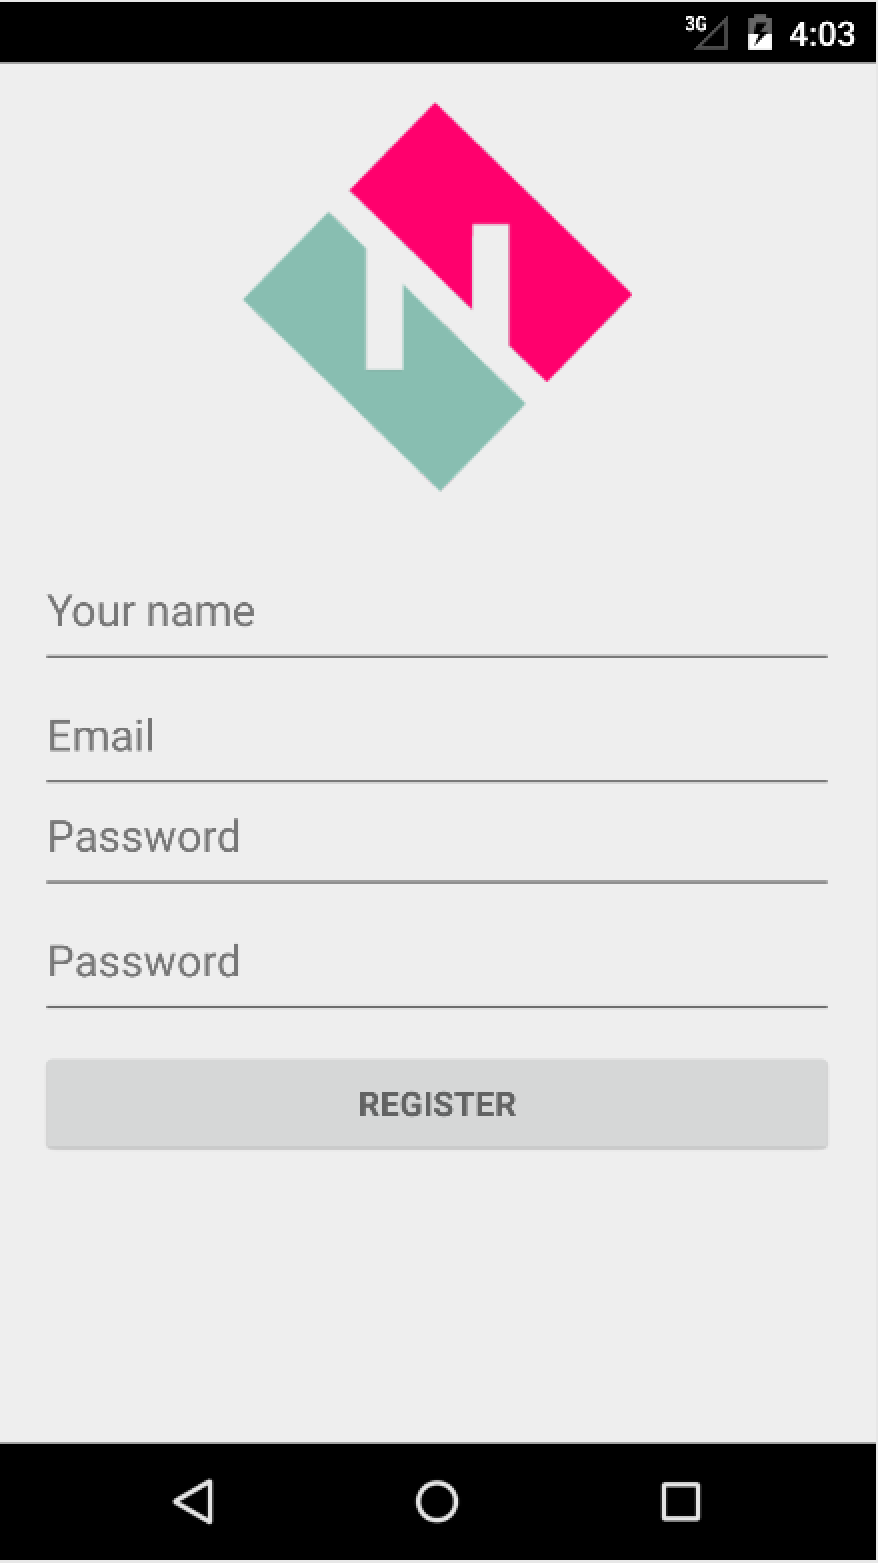
\includegraphics[width=0.9\linewidth]{./Bilder/signUp.png}
\caption{SignUp Screen}
\label{fig:signin}
\end{subfigure}
\caption{}
\label{fig:image2}
\end{figure}

Startet man die App findet man sich zuerst auf einem LogIn/SignUp - Screen wieder. 
Hier kann durch die Eingabe einer g"ultigen Email-adresse und eines Passworts ein Account erstellt, oder sich in einen bestehenden Account eingeloggt werden. 
Die Umsetzung ist schlicht und funktional gehalten. 
Dies kann so "ubernommen werden. 
 
Was erst im Vergleich mit den folgenden Seiten auff"allt, ist dass das Design dieser Seite nicht in das Schema der restlichen App passt. 
Aus Gr"unden der Konsistenz sollte das angepasst werden.

\subsubsection{Start}
\begin{figure}[H]
\begin{center}
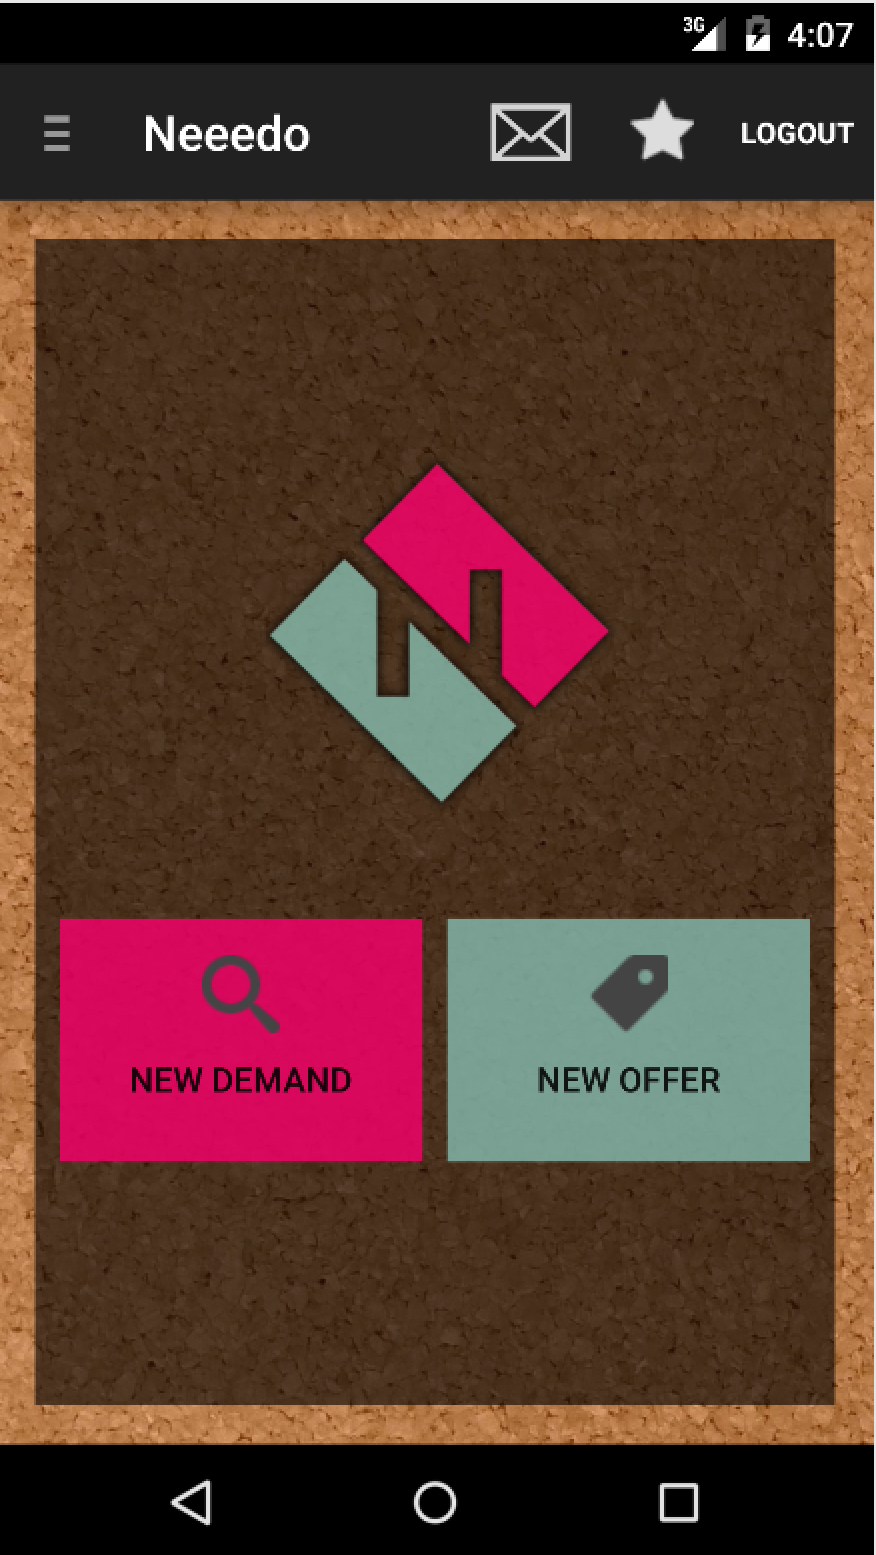
\includegraphics[width=0.45\textwidth]{./Bilder/start.png}
\caption{LandingScreen}
\label{fig:start}
\end{center}
\end{figure}

Loggt man sich in die App ein landet man zuerst auf der hier abgebildeten LandingPage. 
Diese ist schlicht gehalten.
Auf dem halbtransparenten Hintergrund finden sich zwei Button, \enquote{New Demand} und \enquote{New Offer}, die einen wohl zu den Formularen f"uhren mit denen man diese erstellen kann.
Man sieht am oberen Rand des Screens eine Men"uleiste, die einen "BurgerButton" als Men"u, den Schriftzug "Neeedo", ein Briefsymbol als Hinweis auf Nachrichten und einen Logout-Button beinhaltet. 
Dies ist eine (Android-) typische Positionierung f"ur diese  Elemente. 

Der Men"u Button ist dabei der am wenigsten markante Punkt dieses Screens, obwohl man wohl davon ausgehen kann, dass er der Wichtigste ist. 
Der Zugang zum Men"u m"usste markanter sein.

\subsubsection{Men"u}
\begin{figure}[H]
\begin{center}
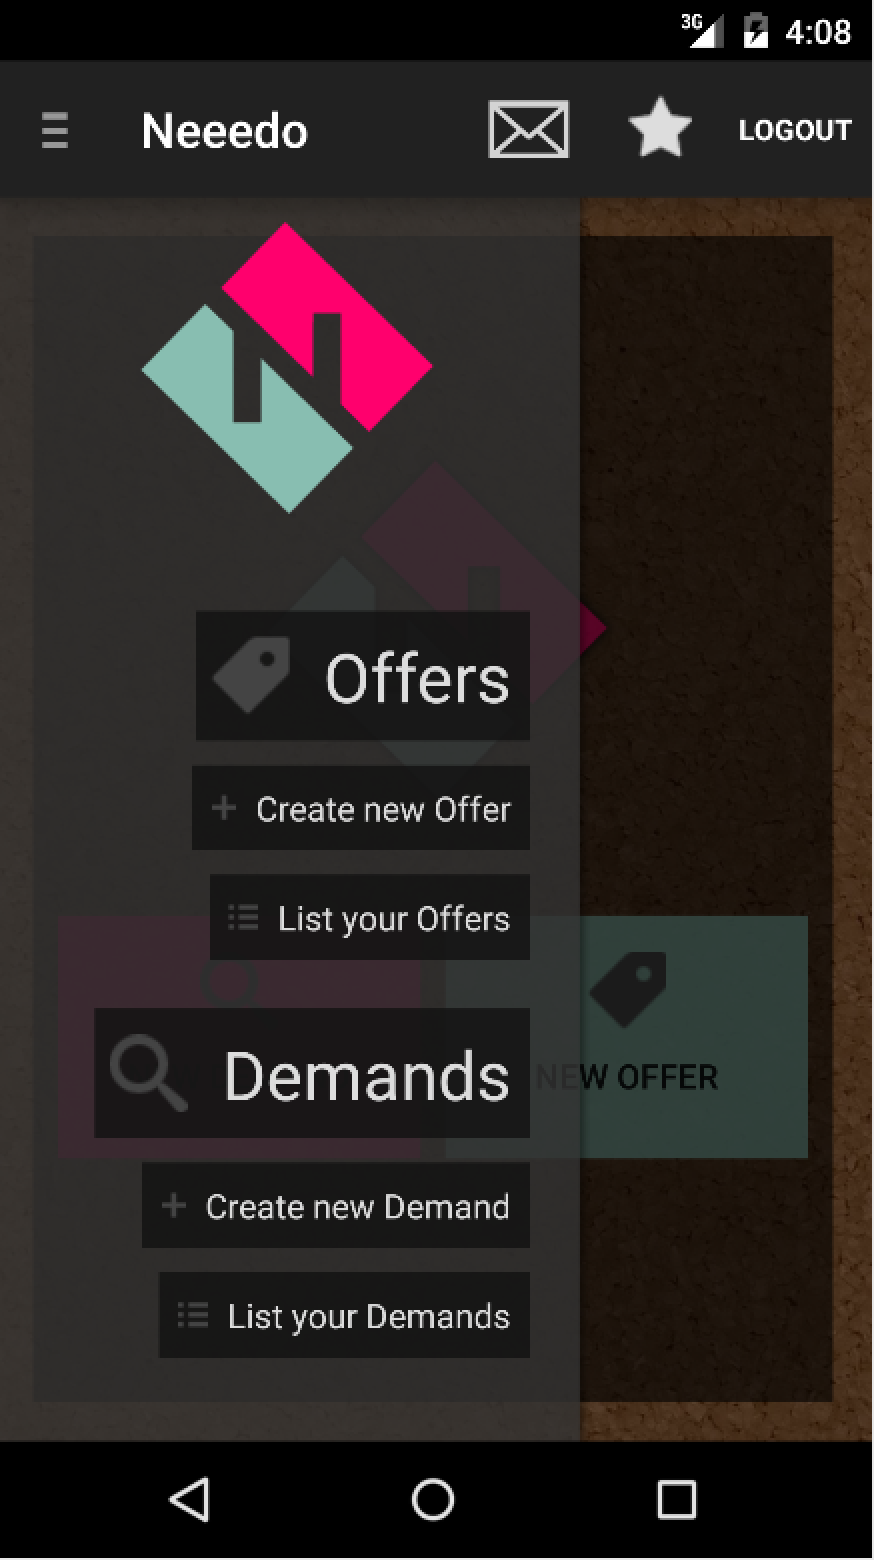
\includegraphics[width=0.45\textwidth]{./Bilder/menu.png}
\caption{Men"u offen}
\label{fig:menu}
\end{center}
\end{figure}

Benutzt man den \enquote{Men"u-Button} "offnet sich das hier abgebildete Men"u.
Dieses bietet, vier Funktionen an: \enquote{Neues Gesuch erstellen}, \enquote{Neues Angebot erstellen}, \enquote{Eigene Angebote auflisten}, \enquote{Eigene Gesuche auflisten}.

Die Umrandung um die Worte, hier, \enquote{Offers} und \enquote{Demands} l"asst vermuten, dass es sich hierbei ebenfalls um Buttons handelt. 
Dies ist jedoch nicht der Fall. 
Es handelt sich hierbei lediglich um Trenner, die das Men"u in drei Sektionen unterteilen.

Betrachtet man sich das Men"u als Ganzes f"allt auf, dass es viel zu viel Platz einnimmt und unn"otig zu sein scheint. 
Um ein solches Men"u zu rechtfertigen m"ssten mehr Funktionen angeboten werden. 

\subsubsection{Agebote und Gesuche erstellen }
\begin{figure}[H]
\begin{subfigure}{0.5\textwidth}
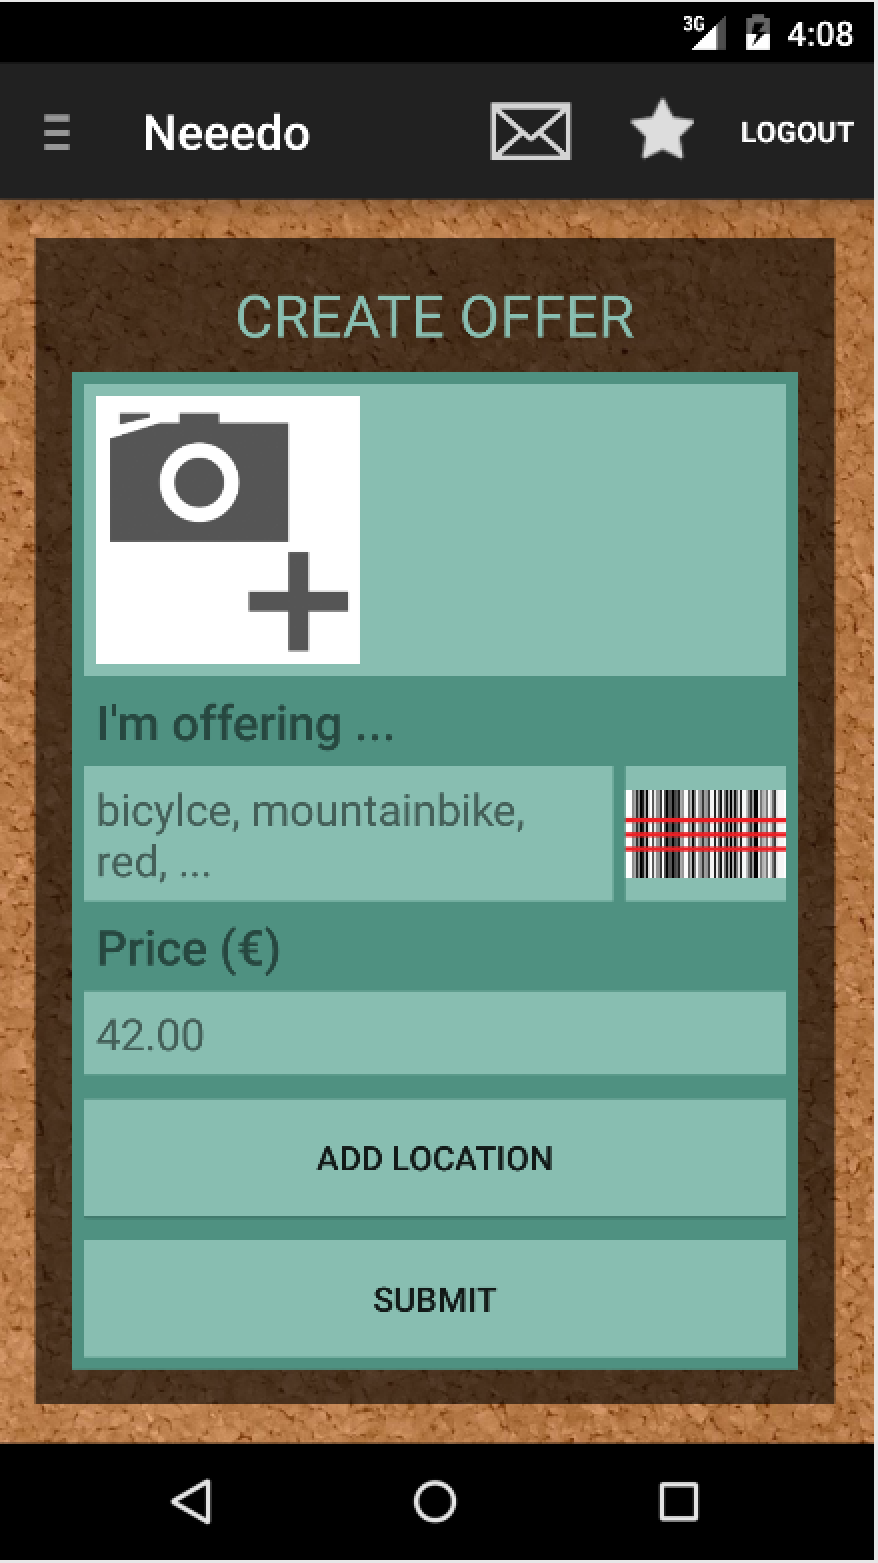
\includegraphics[width=0.9\linewidth]{./Bilder/createOffer.png} 
\caption{Angebot erstellen}
\label{fig:offer}
\end{subfigure}
\begin{subfigure}{0.5\textwidth}
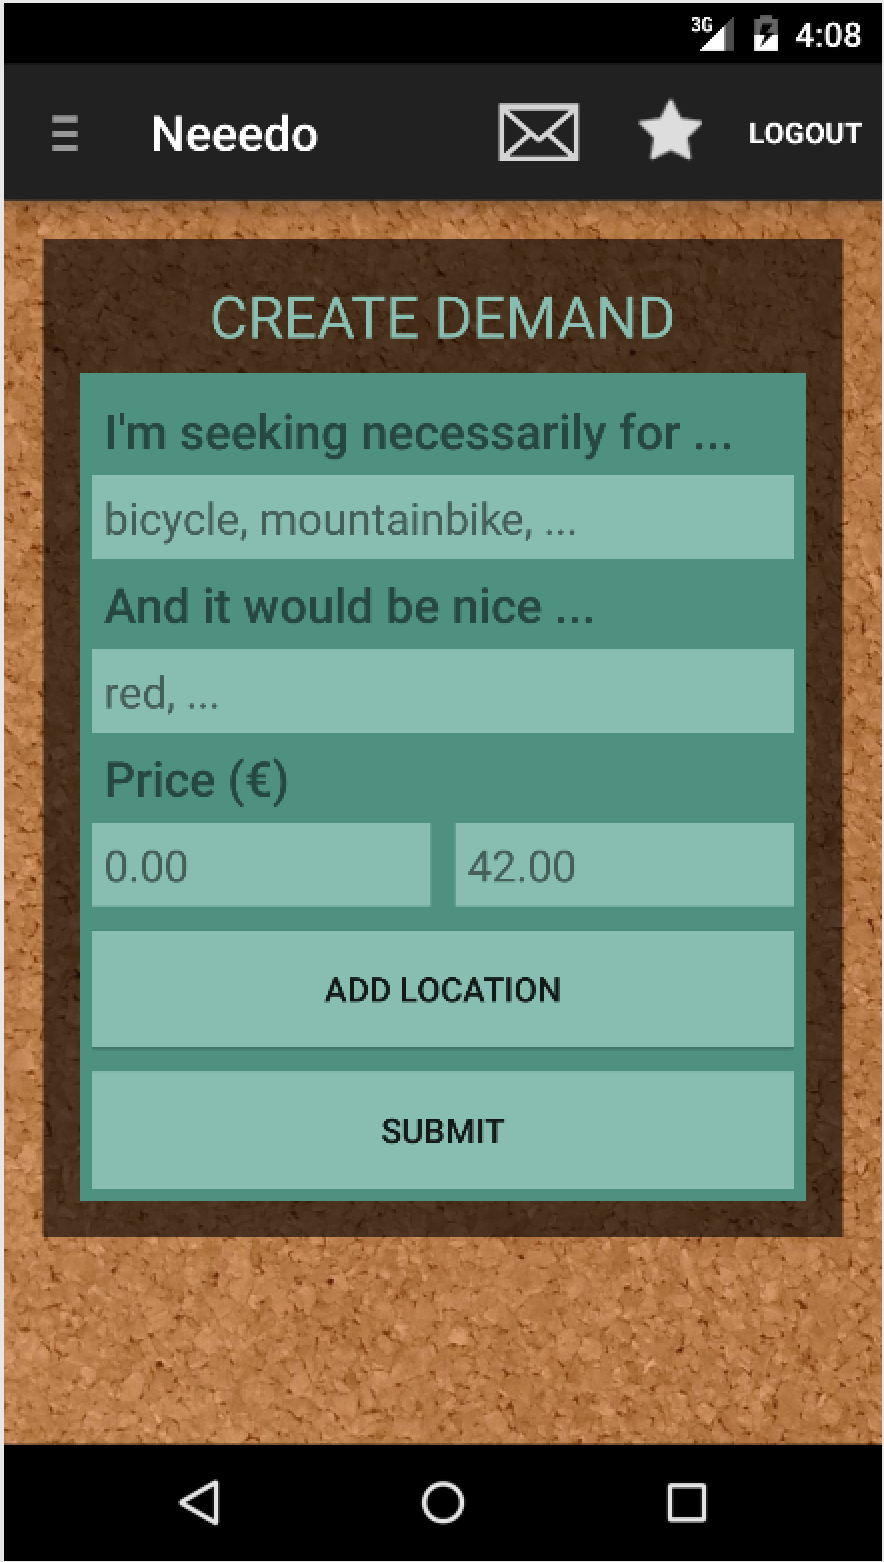
\includegraphics[width=0.9\linewidth]{./Bilder/createDemand.png}
\caption{Gesuch erstellen}
\label{fig:demand}
\end{subfigure}
\caption{}
\label{fig:image4}
\end{figure}

W"ahlt man, entweder im Men"u oder auf dem StartScreen, eine der \enquote{erstellen}-Funktionen aus, landet man auf einer dieser Seiten entsprechend der jeweiligen Auswahl.
Hier wird jeweils ein Formular angezeigt, in dem man eintragen kann was man sucht oder was man anbieten m"ochte. 

Erstellt man ein Angebot/Offer ist es m"oglich Fotos zu hinzuzuf"ugen.
Dies geschieht entweder die Auswahl des Camera-Bildes. 
Dieses ist auf den ersten Blick nicht als Button erkennbar. Dies sollte klarer erkennbar sein. 
Ebenfalls erh"allt man die M"oglichkeit informationen "uber sein Produkt durch das Scannen eines Barcodes zu erhalten. 
Diese Funktionen sind sinnvoll und k"onnten in "ahnlicher Weise "ubernommen werden.

Erstellt man ein Gesuch/Demand, bieter die App keine Zusatzfunktionen an. 
Hier muss das Formular von Hand ausgef"ullt werden.

Beide Formulare besitzen die M"oglichkeit eine Adresse hinzuzuf"ugen, dies geschieht auf einer zus"atzlichen Seite auf der dies durch Auswahl einer Positon auf einer Karte oder ein Suchfeld geschieht.

Befindet man sich auf der Formular-Seite kann man nicht klar erkennen ob man eine Position eingeben muss oder ob es einen Standardwert gibt. 
Dies sollte erkennbar gemacht werden.
 
\subsubsection{Matching}
\begin{figure}[H]
 
\begin{subfigure}{0.5\textwidth}
\includegraphics[width=0.9\linewidth]{./Bilder/matching1.png} 
\caption{Angebot erstellen}
\label{fig:match1}
\end{subfigure}
\begin{subfigure}{0.5\textwidth}
\includegraphics[width=0.9\linewidth]{./Bilder/matching2.png}
\caption{Gesuch erstellen}
\label{fig:match2}
\end{subfigure}
\caption{}
\label{fig:image5}
\end{figure}

Sendet man das auf der \enquote{Gesuch erstellen}-Seite ausgef"ullte Formular ab wird man auf die hier gezeigte \enquote{Matching-View} weitergeleitet. 
Hier werden einem passende Angebote in einer, u.a. aus der App "Tinder" bekannten Stapel-Darstellung pr"sentiert. 
Diese k"onnen entweder durch die Buttons oder durch eine Swipe-Geste nach rechts oder Links verworfen oder als Favorit gespeichert werden. 

Um die gespeicherten Favoriten aufzurufen muss man das Stern-Symbol in der Men"uleiste oben nutzen, im Screen selbst ist keine Weiterleitung m"oglich. 

\subsubsection{\enquote{Eigene} anzeigen}

\begin{figure}[H]
\begin{center}
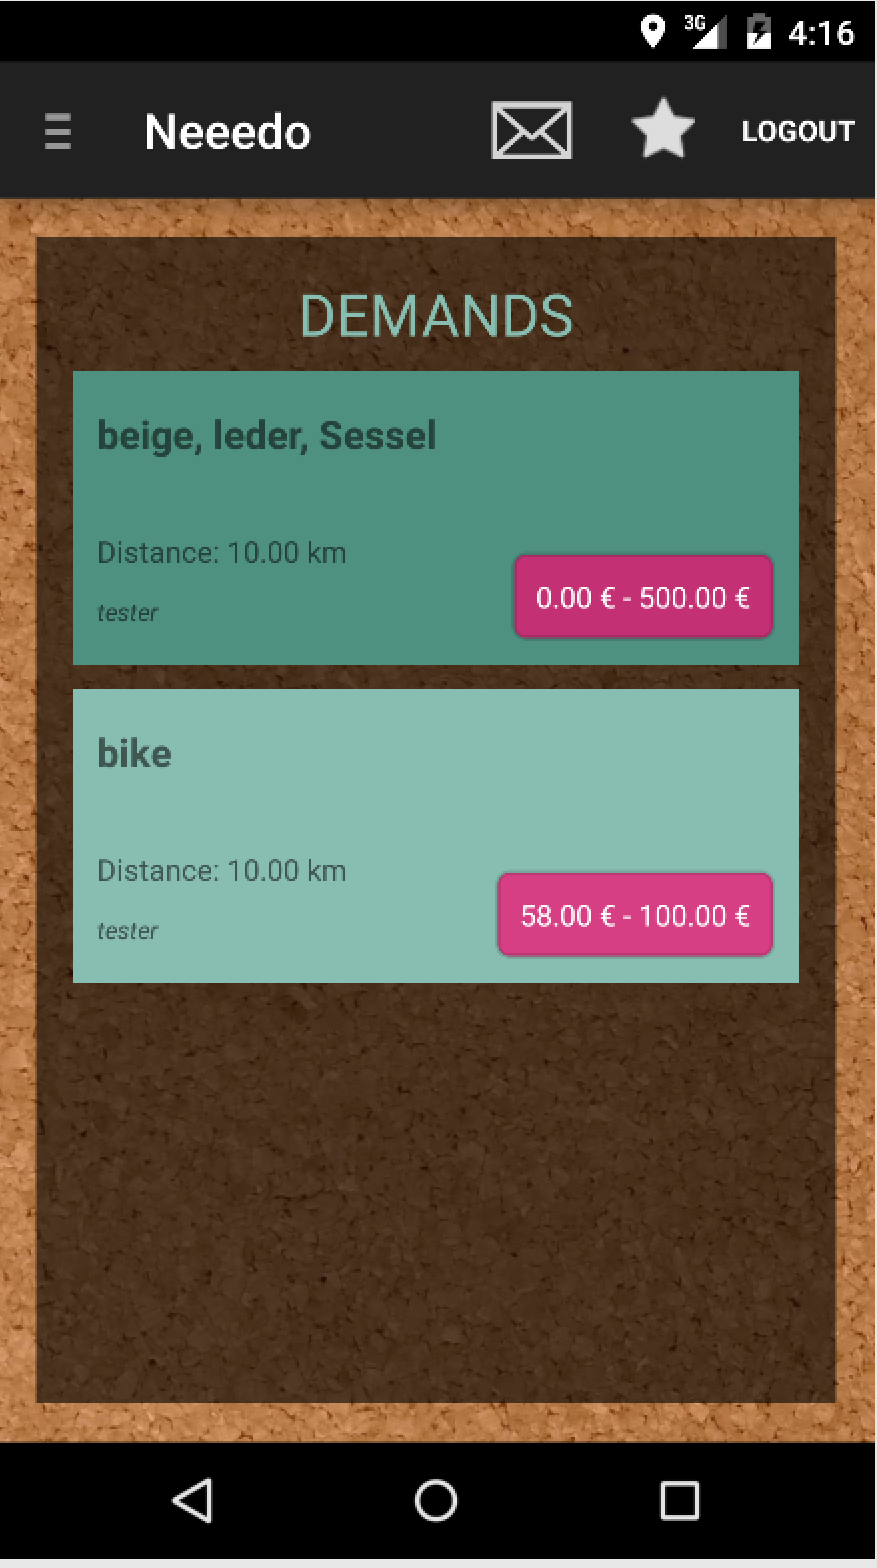
\includegraphics[width=0.45\textwidth]{./Bilder/liste.png}
\caption{Eigene Demands anzeigen}
\label{fig:anzeigen}
\end{center}
\end{figure}

Im Men"u finden sich auch die Funktionen \enquote{eigene Angebote/Gesuche anzeigen}. 
Benutzt man einen dieser Buttons, wird eine Tabelle wie die hier abgebildete pr"asentiert.
Klickt man hier auf eines der aufgef"uhrten Elemente, wird man auf ein Formular "ahnlich dem des \enquote{Erstellens} geleitet, auf dem "Anderungen durchgef"uhrt werden k"onnen. 

\subsection{Fazit}

Dies sind die wichtigsten Funktionen dieser App, weitere wie zum Beispiel der Versand von Nachrichten werden nicht n"aher betrachtet, da hier nur ein Standard Chat zum Einsatz kommt. 

\subsubsection{Positiv}\begin{description}
\item[+] Das Design ist einheitlich 
\item[+] Viele Funktionen k"onnen "ubernommen werden
\end{description}

\subsubsection{Negativ}\begin{description}
\item[-] Nicht alle Buttons k"onnen als solche erkannt werden
\item[-] Elemente k"onnen irrt"umlich f"ur Buttons gehalten werden.
\item[-] Seitenmen"u zu gro"s und unpraktisch 
\item[-] Login nicht im selben Design
\end{description}



% ----------------------------------------------------------------------------------------------------------
% Umsetzung
% ----------------------------------------------------------------------------------------------------------

\section{Umsetzung}
\subsection{Probleme}
\subsection{L"osungen}

% ----------------------------------------------------------------------------------------------------------
% Fazit
% ----------------------------------------------------------------------------------------------------------
\section{Fazit}


% ----------------------------------------------------------------------------------------------------------
% Ausblick
% ----------------------------------------------------------------------------------------------------------
\section{Ausblick}


\end{document}
